\def\due{Monday, 7 September 2020}
\def\zipscript{\texttt{zip -j ps4\_submission.zip src/mnist/nn.py src/spam/spam.py}}
\def\zipscriptalt{\texttt{python zip\_submission.py}}
\def\psetnum{4 }

%%% Change the following flag to toggle between questions or solutions
\ifdefined\solutions {1} \else \def\solutions{2} \fi
%%%%%%%%%%%%%%%%%%%%%%%%%%%%%%%%%%%%%%%%%%%%%%%%%%%%%%%%%%%%%%%%%%%%%%%%%%%%%%%%%%%%%%%%%%%
%                                                                                         %
% PLEASE NOTE THAT THIS DOCUMENT AND IT'S SUB-DOCUMENTS MAY REFER TO "*-sol.tex" FILES    %
% THESE FILES ARE THE SOLUTION FILES CREATED BY THE COURSE STAFF TO FACILITATE COMPILING  %
% BOTH THE PROBLEM SET AND ITS SOLUTIONS IN THE SAME LATEX FOLDER.  STUDENTS WILL NOT     %
% GAIN ACCESS TO THESE "*-sol.tex" FILES UNTIL AFTER THE PROBLEM SET DUE DATE.  IF YOU    %
% ARE RECEIVING ERRORS FROM YOUR LATEX COMPILER ABOUT THESE FILES MISSING, ENSURE THE     %
% LINE IMMEDIATELY PRECEDING THIS STATEMENT IS EXACTLY AS FOLLOWS:                       %
%                                                                                         %
%      \ifdefined\solutions {1} \else \def\solutions{2} \fi                               %
%                                                                                         %
%%%%%%%%%%%%%%%%%%%%%%%%%%%%%%%%%%%%%%%%%%%%%%%%%%%%%%%%%%%%%%%%%%%%%%%%%%%%%%%%%%%%%%%%%%%


\documentclass{article}

\usepackage{graphicx}

\usepackage[utf8]{inputenc}
\usepackage{listings}
\usepackage{xcolor}

\definecolor{codegreen}{rgb}{0,0.6,0}
\definecolor{codegray}{rgb}{0.5,0.5,0.5}
\definecolor{codepurple}{rgb}{0.58,0,0.82}
\definecolor{backcolour}{rgb}{0.95,0.95,0.92}

\lstdefinestyle{mystyle}{
    backgroundcolor=\color{backcolour},   
    commentstyle=\color{codegreen},
    keywordstyle=\color{magenta},
    stringstyle=\color{codepurple},
    basicstyle=\ttfamily\footnotesize,
    breakatwhitespace=false,         
    breaklines=true,                 
    captionpos=b,                    
    keepspaces=true,                 
    numbersep=5pt,                  
    showspaces=false,                
    showstringspaces=false,
    showtabs=false,                  
    tabsize=2
}

\lstset{style=mystyle}

\newcommand{\di}{{d}}
\newcommand{\nexp}{{n}}
\newcommand{\nf}{{p}}
\newcommand{\vcd}{{\textbf{D}}}

\usepackage{hyperref}
\usepackage{nccmath}
\usepackage{mathtools}
\usepackage{graphicx,caption}
\usepackage{enumitem}
\usepackage{epstopdf,subcaption}
\usepackage{psfrag}
\usepackage{amsmath,amssymb,epsf}
\usepackage{verbatim}
% \usepackage[hyphens]{url}
\usepackage{color,soul}
\usepackage{bbm}
\usepackage{listings}
\usepackage{setspace}
\usepackage{float}
\definecolor{Code}{rgb}{0,0,0}
\definecolor{Decorators}{rgb}{0.5,0.5,0.5}
\definecolor{Numbers}{rgb}{0.5,0,0}
\definecolor{MatchingBrackets}{rgb}{0.25,0.5,0.5}
\definecolor{Keywords}{rgb}{0,0,1}
\definecolor{self}{rgb}{0,0,0}
\definecolor{Strings}{rgb}{0,0.63,0}
\definecolor{Comments}{rgb}{0,0.63,1}
\definecolor{Backquotes}{rgb}{0,0,0}
\definecolor{Classname}{rgb}{0,0,0}
\definecolor{FunctionName}{rgb}{0,0,0}
\definecolor{Operators}{rgb}{0,0,0}
\definecolor{Background}{rgb}{0.98,0.98,0.98}
\lstdefinelanguage{Python}{
numbers=left,
numberstyle=\footnotesize,
numbersep=1em,
xleftmargin=1em,
framextopmargin=2em,
framexbottommargin=2em,
showspaces=false,
showtabs=false,
showstringspaces=false,
frame=l,
tabsize=4,
% Basic
basicstyle=\ttfamily\footnotesize\setstretch{1},
backgroundcolor=\color{Background},
% Comments
commentstyle=\color{Comments}\slshape,
% Strings
stringstyle=\color{Strings},
morecomment=[s][\color{Strings}]{"""}{"""},
morecomment=[s][\color{Strings}]{'''}{'''},
% keywords
morekeywords={import,from,class,def,for,while,if,is,in,elif,else,not,and,or
,print,break,continue,return,True,False,None,access,as,,del,except,exec
,finally,global,import,lambda,pass,print,raise,try,assert},
keywordstyle={\color{Keywords}\bfseries},
% additional keywords
morekeywords={[2]@invariant},
keywordstyle={[2]\color{Decorators}\slshape},
emph={self},
emphstyle={\color{self}\slshape},
%
}


\pagestyle{empty} \addtolength{\textwidth}{1.0in}
\addtolength{\textheight}{0.5in}
\addtolength{\oddsidemargin}{-0.5in}
\addtolength{\evensidemargin}{-0.5in}
\newcommand{\ruleskip}{\bigskip\hrule\bigskip}
\newcommand{\nodify}[1]{{\sc #1}}
\newcommand{\points}[1]{{\textbf{[#1 points]}}}
\newcommand{\subquestionpointswritten}[1]{{\textbf{[#1 point(s) Written]}}}
\newcommand{\subquestionpointscoding}[1]{{\textbf{[#1 point(s) Coding]}}}
\newcommand{\subquestionpointscodingandwritten}[1]{{\textbf{[#1 point(s) Written \& Coding]}}}
\newenvironment{answer}{{\bf Answer:} \sf \begingroup\color{red}}{\endgroup}%

\newcommand{\bitem}{\begin{list}{$\bullet$}%
{\setlength{\itemsep}{0pt}\setlength{\topsep}{0pt}%
\setlength{\rightmargin}{0pt}}}
\newcommand{\eitem}{\end{list}}

\setlength{\parindent}{0pt} \setlength{\parskip}{0.5ex}
\setlength{\unitlength}{1cm}

\renewcommand{\Re}{{\mathbb R}}
\newcommand{\R}{\mathbb{R}}
\newcommand{\what}[1]{\widehat{#1}}

\renewcommand{\comment}[1]{}
\newcommand{\mc}[1]{\mathcal{#1}}
\newcommand{\half}{\frac{1}{2}}

\def\KL{D_{KL}}
\def\xsi{x^{(i)}}
\def\ysi{y^{(i)}}
\def\zsi{z^{(i)}}
\def\E{\mathbb{E}}
\def\calN{\mathcal{N}}
\def\calD{\mathcal{D}}
\def\slack{\url{http://xcs229i-scpd.slack.com/}}

\usepackage{tikz}
\usepackage{bbding}
\usepackage{pifont}
\usepackage{wasysym}
\usepackage{amssymb}




\begin{document}

\pagestyle{myheadings} \markboth{}{XCS229i Problem Set \psetnum}

\ifnum\solutions=1{
{\huge\noindent XCS229i Problem Set \psetnum (Solutions)}
} \else {
\huge\noindent XCS229i Problem Set \psetnum
} \fi

\ruleskip

{\bf Due {\due }.}

\medskip


{\bf Guidelines}
\begin{enumerate}
    \item These questions require thought, but do not require long answers. Please be as concise as possible.
    \item If you have a question about this homework, we encourage you to post your question on our Slack channel, at \slack
    \item Familiarize yourself with the collaboration and honor code policy before starting work.
    \item For the coding problems, you may not use any libraries except those defined in the provided started code. In particular, ML-specific libraries such as \texttt{scikit-learn} are not permitted.
\end{enumerate}


\smallskip

{\bf Submission Instructions} \\~\\
{\bf Written Submission:}
All students must submit an electronic PDF version of the written questions. We highly recommend typesetting your solutions via \LaTeX, though it is not required. If you choose to hand write your responses, please make sure they are well organized and legible when scanned. The source \LaTeX for all problem sets is available on GitHub.\\~\\
{\bf Coding Submission:}
All students must also submit a zip file of their source code.
Create a submission using the following bash command:\\\\
\small{\zipscript}\\\\ 
You should make sure to (1) restrict yourself to only using libraries included in the starter code, and (2) make sure your code runs without errors.
Your submission will be evaluated by the auto-grader using a private test set and will be used for verifying the outputs reported in the writeup.\\~\\~\\

\smallskip

{\bf Honor code:} We strongly encourage students to form study
groups. Students may discuss and work on homework problems in
groups. However, each student must write down the solutions independently,
and without referring to written notes from the joint session. In other
words, each student must understand the solution well enough in order to
reconstruct it by him/herself. In addition, each student should write on
the problem set the set of people with whom s/he collaborated.
Further, because we occasionally reuse problem set questions from previous
years, we expect students not to copy, refer to, or look at the solutions
in preparing their answers. It is an honor code violation to intentionally
refer to a previous year's solutions.



\begin{enumerate}[wide, labelwidth=!, labelindent=0pt]

\clearpage
\item \points{20} {\bf Spam classification}

In this problem, we will use the Naive Bayes algorithm and an SVM to
build a spam classifier.

In recent years, spam on electronic media has been a growing concern.  Here, we'll build a classifier to distinguish
between real messages, and spam messages. For this class, we will be building a classifier to detect SMS spam messages. We will be using an SMS spam dataset developed by Tiago A. Almedia and José María Gómez Hidalgo which is publicly available on \url{http://www.dt.fee.unicamp.br/~tiago/smsspamcollection} \footnote{Almeida, T.A., Gómez Hidalgo, J.M., Yamakami, A. Contributions to the Study of SMS Spam Filtering: New Collection and Results.  Proceedings of the 2011 ACM Symposium on Document Engineering (DOCENG'11), Mountain View, CA, USA, 2011.}

We have split this dataset into training and testing sets and have included them in this assignment as \texttt{src/spam/spam\_train.tsv} and \texttt{src/spam/spam\_test.tsv}. See \texttt{src/spam/spam\_readme.txt} for more details about this dataset. Please refrain from redistributing these dataset files. The goal of this assignment is to build a classifier from scratch that can tell the difference the spam and non-spam messages using the text of the SMS message.

\begin{enumerate}
  \item \subquestionpointscoding{5}
Implement code for processing the the spam messages into numpy arrays that can be fed into machine learning models. Do this by completing the \texttt{get\_words}, \texttt{create\_dictionary}, and \texttt{transform\_text} functions within our provided \texttt{src/spam.py}. Do note the corresponding comments for each function for instructions on what specific processing is required.

The provided code will then run your functions and save the resulting dictionary into \texttt{spam\_dictionary} and a sample of the resulting training matrix into\\
\texttt{spam\_sample\_train\_matrix}.\\[50pt]
  \ifnum\solutions=1 {
    \input{spam/01-input-processing-sol}
  } \fi

  \item \subquestionpointscoding{5}
In this question you are going to implement a naive Bayes classifier for spam
classification with {\bf multinomial event model} and Laplace smoothing.

Code your implementation by completing the \texttt{fit\_naive\_bayes\_model}
and \\\texttt{predict\_from\_naive\_bayes\_model} functions in
\texttt{src/spam/spam.py}.

Now \texttt{src/spam/spam.py} should be able to train a Naive Bayes model,
compute your prediction accuracy and then save your resulting predictions
to \texttt{spam\_naive\_bayes\_predictions}.

In your writeup, report the accuracy of the trained model on the \textbf{test set}.

{\bf Remark.} If you implement naive Bayes the straightforward way, you will find
that the computed $p(x|y) = \prod_i p(x_i | y)$ often equals zero.  This is
because $p(x|y)$, which is the product of many numbers less than one, is a very
small  number. The standard computer representation of real numbers cannot
handle numbers that are too small, and instead rounds them off to zero.  (This
is called  ``underflow.'')  You'll have to find a way to compute Naive Bayes'
predicted  class labels without explicitly representing very small numbers such
as $p(x|y)$.
[\textbf{Hint:} Think about using logarithms.]\\[50pt]
  \ifnum\solutions=1 {
    \input{spam/02-naive-bayes-sol}
  } \fi

  \item \subquestionpoints{5}
Intuitively, some tokens may be particularly indicative of an SMS being
in a particular class.  We can try to get an informal sense of how indicative
token $i$ is for the SPAM class by looking at:
\begin{equation*}
  \log \frac{p(x_j = i| y=1)}{p(x_j = i|y=0)}
  = \log\left(\frac{P(\hbox{token $i$} | \hbox{email is SPAM})}
    {P(\hbox{token $i$} | \hbox{email is NOTSPAM})}\right).
\end{equation*}

Complete the \texttt{get\_top\_five\_naive\_bayes\_words} function within the provided code using the above formula in order to obtain the 5 most indicative tokens.

Report the top five words in your writeup.\\[50pt]
  \ifnum\solutions=1 {
    \input{spam/03-five-best-sol}
  } \fi

  \item \subquestionpoints{5}
Support vector machines (SVMs) are an alternative machine learning model that we discussed in class.
We have provided you an SVM implementation (using a radial basis function (RBF) kernel) within \texttt{src/spam/svm.py} (You should not need to modify that code).

One important part of training an SVM parameterized by an RBF kernel (a.k.a Gaussian kernel) is choosing an appropriate kernel radius parameter.

Complete the \texttt{compute\_best\_svm\_radius} by writing code to compute the best SVM radius which maximizes accuracy on the validation dataset. Report the best kernel radius you obtained in the writeup.\\[50pt]
  \ifnum\solutions=1 {
    \input{spam/04-svm-sol}
  } \fi
\end{enumerate}


\clearpage
\item \points{20} {\bf Neural Networks: MNIST image classification}

In this problem, you will implement a simple neural network
to classify grayscale images of handwritten digits (0 - 9) from
the MNIST dataset. The dataset contains 60,000 training images and
10,000 testing images of handwritten digits, 0 - 9. Each image is
28$\times$28 pixels in size, and is generally represented as a flat
vector of 784 numbers. It also includes labels for each example, a number
indicating the actual digit (0 - 9) handwritten in that image. A sample of
a few such images are shown below.

\begin{center}

\includegraphics[scale=0.5]{mnist/mnist_plot}
\end{center}


The data and starter code for this problem can be found in

\begin{itemize}
\item \texttt{src/mnist/nn.py}
\item \texttt{src/mnist/images\_train.csv}
\item \texttt{src/mnist/labels\_train.csv}
\item \texttt{src/mnist/images\_test.csv}
\item \texttt{src/mnist/labels\_test.csv}
\end{itemize}

The starter code splits the set
of 60,000 training images and labels into a set of 50,000 examples as
the training set, and 10,000 examples for dev set.

To start, you will implement a neural network with a single hidden layer
and cross entropy loss, and train it with the provided data set. Use the
sigmoid function as activation for the hidden layer, and softmax function
for the output layer. Recall that for a single example $(x, y)$, the cross
entropy loss is:
$$CE(y, \hat{y}) = - \sum_{k=1}^K y_k \log \hat{y_k},$$
where $\hat{y} \in \mathbb{R}^{K}$ is the vector of softmax outputs
from the model for the training example $x$,
and $y \in \mathbb{R}^{K}$ is the ground-truth vector for the training example
$x$ such that $y = [0,...,0,1,0,...,0]^\top$ contains a single 1 at the
position of the correct class (also called a ``one-hot'' representation).

For $\nexp$ training examples, we average the cross entropy loss over the $\nexp$ examples.
  \begin{equation*}
  J(W^{[1]},W^{[2]},b^{[1]},b^{[2]}) = \frac{1}{\nexp}\sum_{i=1}^\nexp CE(y^{(i)}, \hat{y}^{(i)}) = - \frac{1}{\nexp}\sum_{i=1}^\nexp \sum_{k=1}^K y_k^{(i)} \log \hat{y}_k^{(i)}.
  \end{equation*}
The starter code already converts labels into one hot representations for you.

Instead of batch gradient descent or stochastic gradient descent, the common practice
is to use mini-batch gradient descent for deep learning tasks. In this case, the
cost function is defined as follows:

  \begin{equation*}
  J_{MB} = \frac{1}{B}\sum_{i=1}^{B}CE(y^{(i)}, \hat{y}^{(i)})
  \end{equation*}
where $B$ is the batch size, i.e. the number of training example in each mini-batch. 

\begin{enumerate}
  \item \subquestionpointscoding{12} 

Implement both forward-propagation and back-propagation for the above loss function.
Initialize the weights of the network by sampling values from a standard normal
distribution. Initialize the bias/intercept term to 0.
Set the number of hidden units to be 300, and learning rate to be 5. Set $B = 1,000$
(mini batch size). This means that we train with 1,000 examples in each iteration.
Therefore, for each epoch, we need 50 iterations to cover the entire training data.
The images are pre-shuffled. So you don't need to randomly sample the data, and can
just create mini-batches sequentially.


Train the model with mini-batch gradient descent
as described above. Run the training for 30 epochs. At the end of each epoch, calculate
the value of loss function averaged over the entire training set.  To verify a correct implementation, consider plotting the average loss (y-axis) against the number of epochs (x-axis). In the same image, plot the value of the loss function averaged over the dev set, and plot it against the number of epochs.

Similarly, consider plotting the accuracy (on y-axis) over the training set,
measured as the fraction of correctly classified examples, versus the number of epochs
(x-axis). In the same image, plot the accuracy over the dev set versus number of epochs.

Also, at the end of 30 epochs, save the learnt parameters (i.e all the weights and biases)
into a file, so that next time you can directly initialize the parameters with
these values from the file, rather than re-training all over. You do NOT need to
submit these parameters.


\textbf{Hint:} Be sure to vectorize your code as much as possible! Training can be
very slow otherwise.

\clearpage\newpage

You plots should look similar to the following:

\begin{figure}[H]
    \centering
    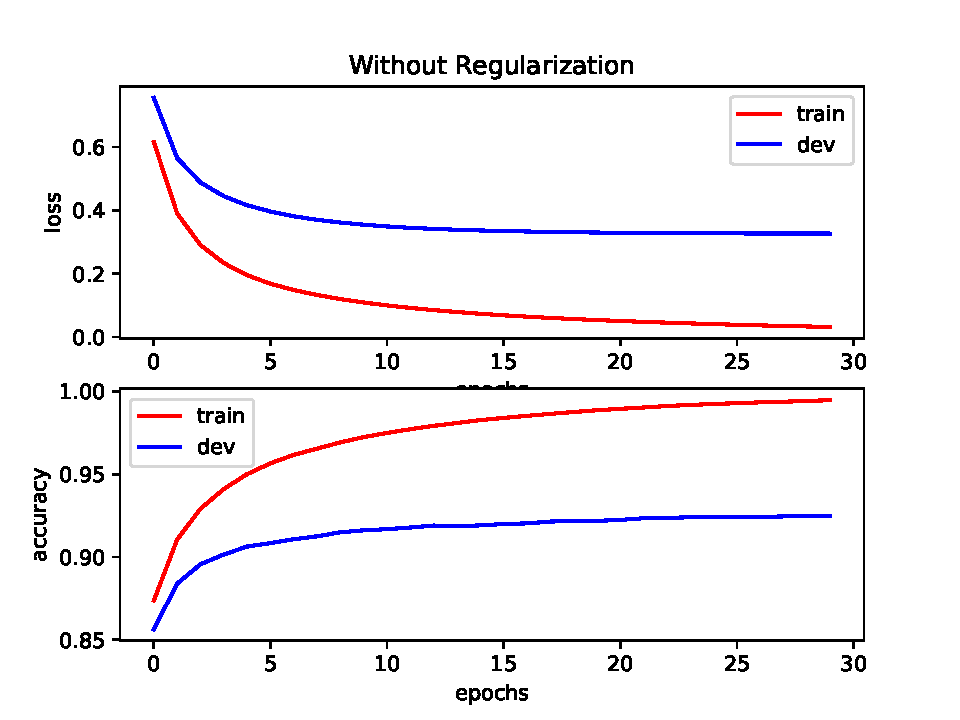
\includegraphics[scale=0.75]{mnist/src/baseline.pdf}
\end{figure}


\ifnum\solutions=1 {
  \input{mnist/01-unregularized-sol}
} \fi

  \item \points{5} Now add a regularization term to your cross entropy loss.
The loss function will become \begin{equation*}
  J_{MB} = \left(\frac{1}{B}\sum_{i=1}^{B}CE(y^{(i)}, \hat{y}^{(i)})\right) + \lambda \left(||W^{[1]}||^2 + ||W^{[2]}||^2 \right)
  \end{equation*}

Be careful not to regularize the bias/intercept term.
Set $\lambda$ to be 0.0001. Implement the regularized version and plot the same
figures as part (a). Be careful NOT to include the regularization term to measure
the loss value for plotting (i.e., regularization should only be used for gradient calculation for
the purpose of training).

\textbf{Submit the two new plots obtained with regularized training (i.e loss (without regularization term) vs epoch, and accuracy vs epoch) in your writeup.}

\textbf{Compare the plots obtained from the regularized model with the plots obtained
from the non-regularized model, and summarize your observations in a couple of sentences.}

As in the previous part, save the learnt parameters (weights and biases) into a
different file so that we can initialize from them next time.

\clearpage\newpage
You plots should look similar to the following:

\begin{figure}[H]
    \centering
    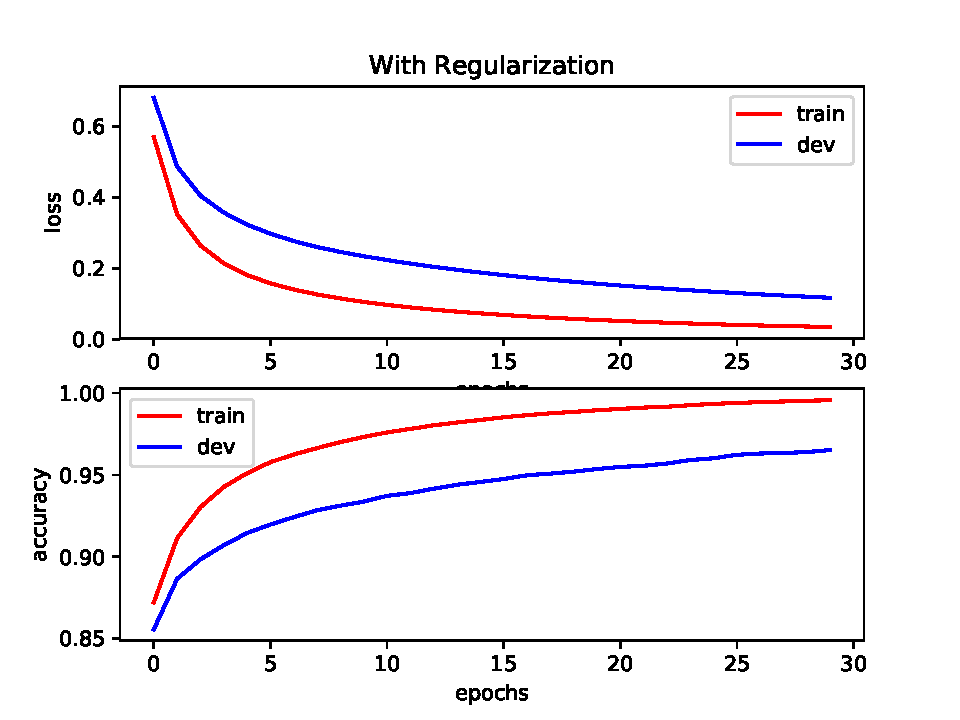
\includegraphics[scale=0.75]{mnist/src/regularized.pdf}
\end{figure}

\ifnum\solutions=1 {
  \input{mnist/02-regularized-sol}
} \fi


  \item \points{3}
All this while you should have stayed away from the test data completely. Now that
you have convinced yourself that the model is working as expected (i.e, the
observations you made in the previous part matches what you learnt in class
about regularization), it is finally time to measure the model performance on
the test set. Once we measure the test set performance, we report it (whatever
value it may be), and NOT go back and refine the model any further.

Initialize your model from the parameters saved in part (a) (i.e, the non-regularized
model), and evaluate the model performance on the test data. Repeat this using the
parameters saved in part (b) (i.e, the regularized model).

Report your test accuracy for both regularized model and non-regularized model.  
Briefly (in one sentence) explain why this outcome makes sense"
You should have accuracy close to 0.92870 without regularization, and 0.96760 with regularization.
Note: these accuracies assume you implement the code with the matrix dimensions as specified in
the comments, which is not the same way as specified in your code. Even if you do not precisely these
numbers, you should observe good accuracy and better test accuracy with regularization.


\ifnum\solutions=1 {
  \input{mnist/03-compare-sol}
} \fi

 \end{enumerate}



\end{enumerate}

\end{document}
